\documentclass[a4paper]{article}

\usepackage{graphicx}
\usepackage{amsmath}
\usepackage{geometry}
\usepackage{tikz}
\usetikzlibrary{backgrounds}

\graphicspath{{../images/}}

\title{\textbf{HABIB UNIVERSITY} \\
\textbf{CS 412: Algorithms: Design and Analysis}
}
\author{Hard-Algorithms \\ Shortest path problem}
\date{Spring 2022}

\begin{document}
\maketitle
\section{Group Members:}
\begin{itemize}
    \item Alisha Momin - am05757
    \item Lama Imam - li06072
    \item Muhammad Hammad Maqdoom - mm05534
    \item Fatima Nasir Khan - fn05458

\end{itemize}
\section{Project Idea:}
We will be implementing graph algorithms to find the shortest path for directed and undirected graph having positive or negative weighted edges for cyclic and acyclic graphs. Our project will comprise of a comprehensive report detailing the implementations and time complexity analysis as well as performance analysis of the algorithms we have chosen.

\section{What is shortest path problem?}
In graph theory, the shortest path problem is the problem that is mainly discussed about finding a shortest path between two vertices (or nodes) in a graph such that the total cost of traversing or sum of the weights of the edges traversed is minimized.
\section{Algorithms to solve shortest path problem:}
The following algorithms are used for solving the shortest path problem:
\begin{itemize}
\item Dijkstra algorithm
\item Bellman–Ford
\item A* search algorithm
\item Floyd–Warshall algorithm
\item Johnson’s algorithm
\item Viterbi algorithm
\end{itemize}
The main focus of this report will be on Dijkstra, Bellman–Ford and Floyd- Warshall algorithm.

\section{Implementation and Analysis:}

\begin{itemize}
    \item[1.] Application and analysis of BFS in finding the shortest path in undirected and directed graph. Since BFS will not work on weighted graphs since the path with the fewest edges may not be the shortest if the edges it contains are expensive, we will analyze another algorithm.
    \begin{center}
        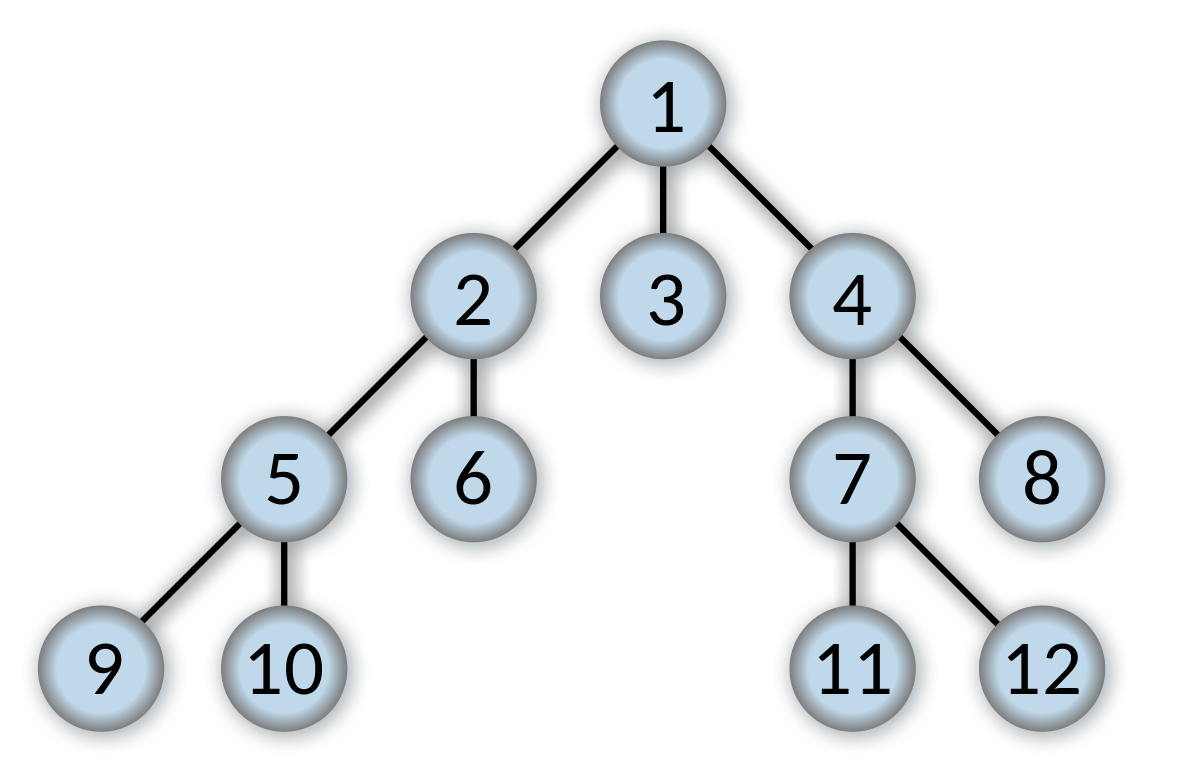
\includegraphics[width=10cm]{images/bfs.png} 
    \end{center}
\item[2.] To find the shortest path in graph with weighted positive edges, we will be implementing and analyzing Dijkstra algorithm. Since Dijkstra algorithm solves the shortest-path problem for any weighted, directed graph with non-negative weights. It can handle graphs consisting of cycles but not for the negative weight. \begin{center}
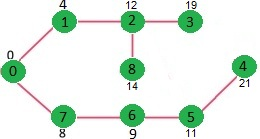
\includegraphics[width=10cm]{images/DIJ5.jpg}
\end{center}
\item[3.] To find the shortest path in graph with weighted negative edges, we will be implementing and analyzing Bellman–Ford algorithm. Since Bellman Ford algorithm helps us find the shortest path from a vertex to all other vertices of a weighted graph as it can work with graphs in which edges can have negative weights. \begin{center}
    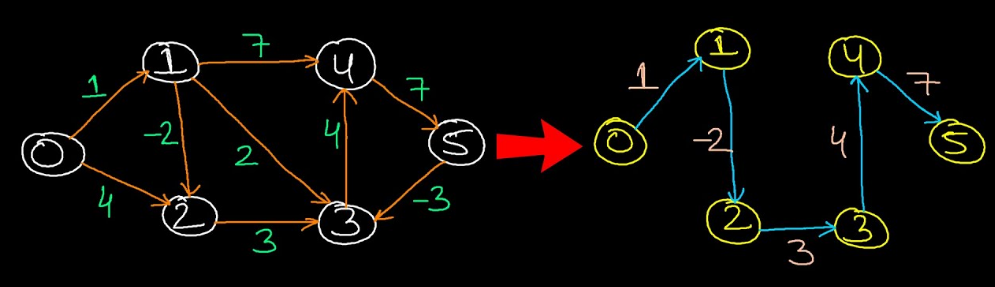
\includegraphics[width=10cm]{images/bellmans.PNG}
\end{center}
\item[4.] For acyclic weighted graph, we will be implementing and analyzing Floyd – Warshall algorithm. Since this algorithm is used to find the shortest paths in a directed weighted graph with positive or negative edge weights (but with no negative cycles). \begin{center}
    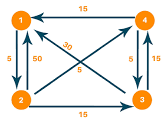
\includegraphics[width=10cm]{images/floyd.PNG} 
\end{center}
\end{itemize}
\end{document}